\chapter{Introduction}

\begin{quote}
    Complex (and useful) behavior need not necessarily be a product of an extremely complex control system. Rather, complex behavior may simply be the reflection of a complex environment. It may be an observer who ascribes complexity to an organism - not necessarily its designer.\\
     \textcite{simon1969sciences}.
\end{quote}


This thesis is an exploration of the methods in adaptive sampling for autonomous underwater vehicles, implemented with a scientific goal in mind. Adaptive sampling in the ocean is as old as fishermen finding new locations to cast their nets. As humans have evolved, so have our methods for sampling the ocean, and pioneers, such as Fridtjof Nansen, Harald U. Sverdrup and Walter Munk paved the way for modern ocean science. In the digital era, robots are increasingly replacing humans in the oceanic domain, thus, a conundrum arises; what is the most effective use of robots in the ocean? Most autonomous operation is dependent on a plan being made before the mission is started. This limits the ability of the autonomous agent to explore the environment based on the measurements it makes along its path leading to under-sampling of interesting regions and oversampling of redundant information. Since it is hard to know \textit{a priori} where the region of interest is, especially in the ocean, it can be advantageous to implement adaptive behaviour on the autonomous agents.



\section{Thesis outline}

\begin{figure}
    \centering
    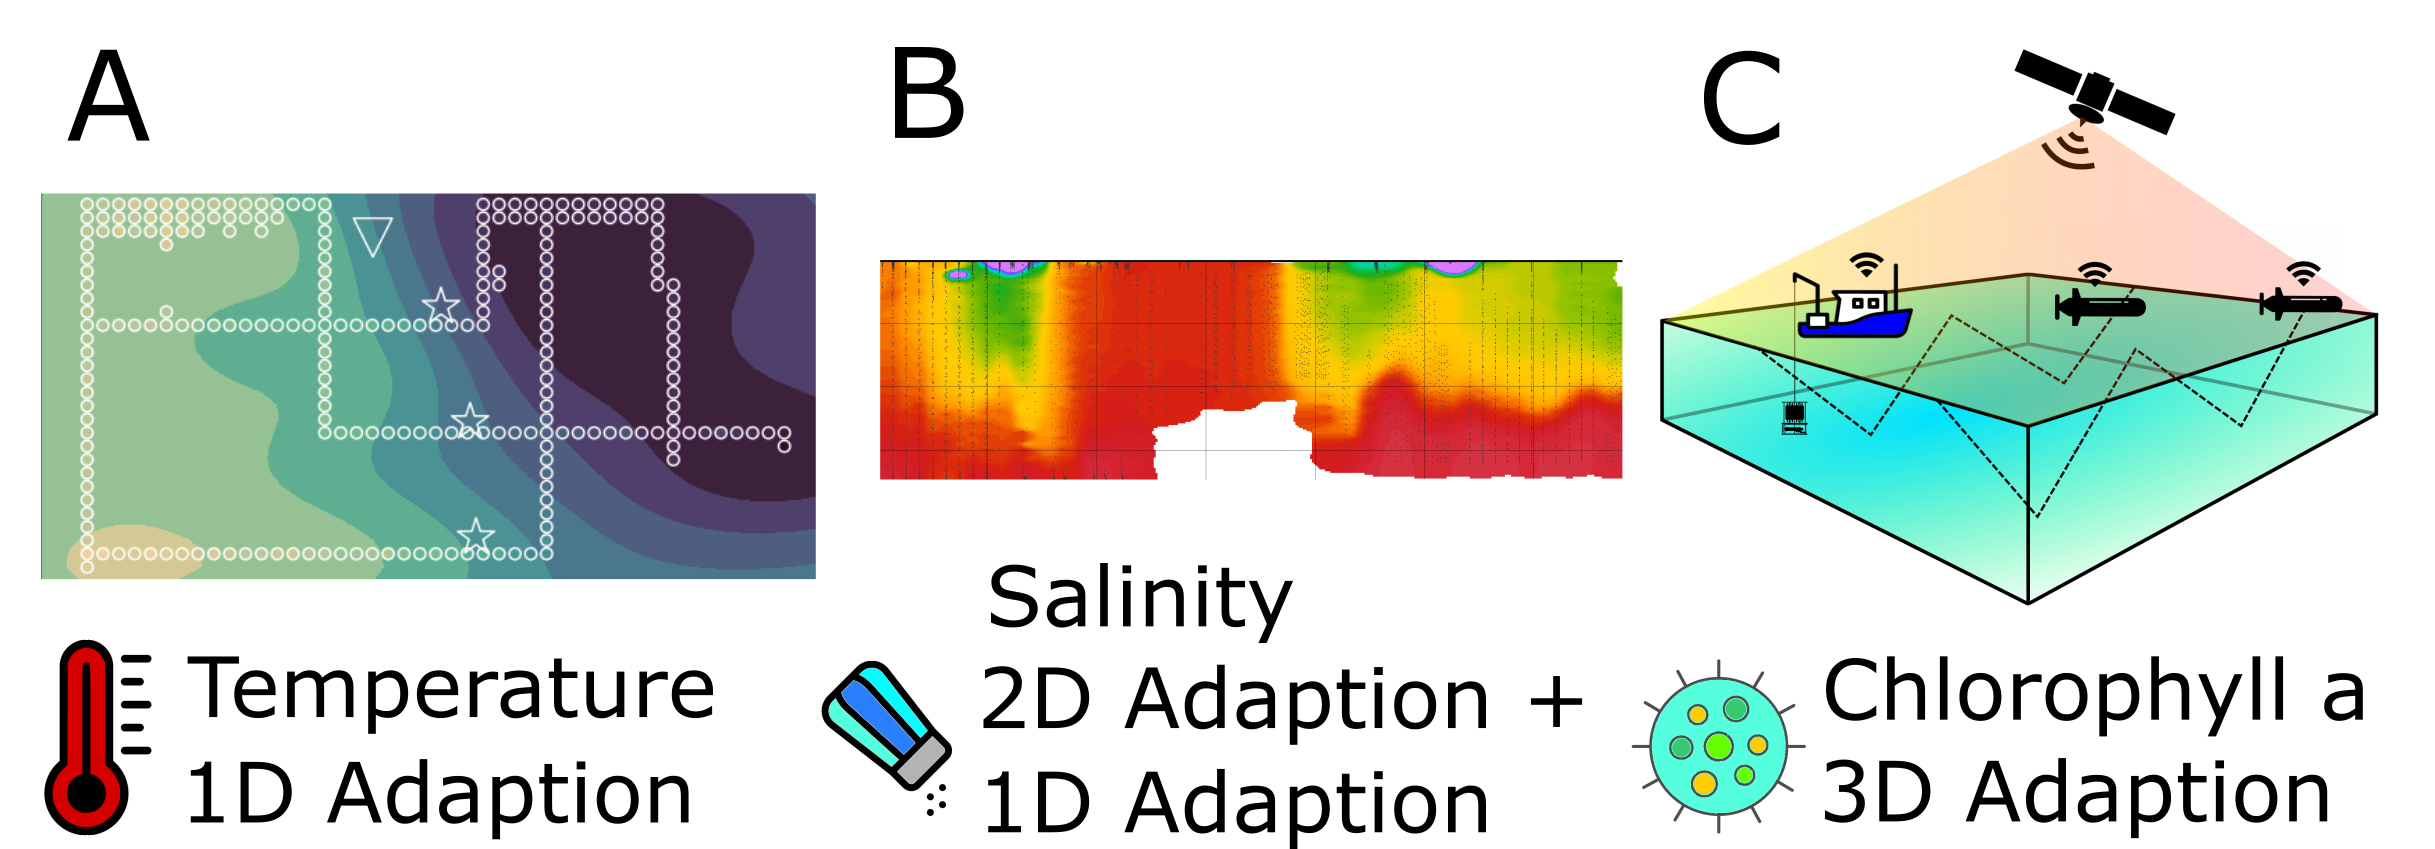
\includegraphics[width=\textwidth]{figures/papersabc.png}
    \caption{Conceptual overview of \textbf{papers A, B and C}. With (A) a temperature contour plot over the polar front, the (B) vertical salinity distribution in and outside the Douro river, and the (C) conceptual overview over the mutli-vehicle operation in \textbf{paper C}. }
    \label{fig:papers}
\end{figure}
The main contribution of this work is related to the applied implementations of adaptive sampling strategies using \acrlong{auv}s in the upper water column. Applying field knowledge and statistical modelling as a base for decision making, methods were implemented and field tested in open ocean (Paper \textbf{A}) and the Arctic (Papers \textbf{A} and \textbf{C}). Additionally, a full integration and field testing campaign was completed remotely, due to the 2020 global Coronavirus pandemic (Paper \textbf{B}).

\subsection*{List of Included Papers}
\begin{itemize}
    \item[\textbf{A:}] \textbf{\textit{Peer-reviewed Journal Article}}\\ \textbf{Tore Mo-Bjørkelund}, Eivind Kolås, Ilker Fer, and Martin Ludvigsen. \textbf{Adaptive tracking of the Barents Sea polar front using an autonomous underwater vehicle}. \textcolor{red}{TODO: Journal etc, JFR}
    
    \item[\textbf{B:}] \textbf{\textit{Peer-reviewed Journal Article}}\\ \textbf{Tore Mo-Bjørkelund}, Renato Mendes, Francisco López-Castejón, and Martin Ludvigsen. \textbf{Adaptive ocean gradient tracking using an autonomous underwater vehicle with a boundless model} \textcolor{red}{JOE, journal etc}
    
    \item[\textbf{C:}] \textbf{\textit{Peer-reviewed Journal Article}}\\ \textbf{Tore Mo-Bjørkelund}, Sanna Majaneva, Glaucia M. Fragoso, Geir Johnsen, and Martin Ludvigsen. \textbf{Multi vehicle adaptive 3D mapping for targeted ocean sampling} \textcolor{red}{scientific reports etc.}
    
    \item[\textbf{D:}]  \textbf{\textit{Peer-reviewed Journal Article}}\\ Yaolin Ge, \textbf{Tore Mo-Bjørkelund}, and Jo Eidsvik. \textbf{3D Adaptive AUV Sampling for Classification of Water Masses}
    
    \item[\textbf{E:}] \textbf{\textit{Technical note}}\\  Eivind H. Kolås, \textbf{Tore Mo-Bjørkelund}, and Ilker Fer. \textbf{Turbulence measurements from a light autonomous underwater vehicle}
    
    \item[\textbf{F:}] \textbf{\textit{Conference paper}}\\ \textbf{Tore Mo-Bjørkelund}, Trygve O. Fossum, Petter Norgren, and Martin Ludvigsen. \textbf{Hexagonal grid graph as a basis for adaptive sampling of ocean Gradients using AUVs}. In Global Oceans 2020: Singapore–US Gulf Coast (pp. 1-5). IEEE.
    
    \item[\textbf{G:}] \textbf{\textit{Conference paper}}\\ \textbf{Tore Mo-Bjørkelund}, Petter Norgren, and Martin Ludvigsen. \textbf{Simulation and forecasting of ice drift as a tool for autonomous under ice operations}. In 2020 IEEE/OES Autonomous Underwater Vehicles Symposium (AUV) (pp. 1-6). IEEE.
    
\end{itemize}